\documentclass[12pt]{article}
\usepackage{polyglossia}
\setdefaultlanguage{spanish}
\setotherlanguage{english}
\usepackage{fontspec}
\usepackage{savesym} % Renames commands for conflicted packages
\usepackage[export]{adjustbox}
\usepackage{amsfonts, amsmath, amssymb}
\usepackage{annotate-equations}
\usepackage{bm}
\usepackage{bookmark}
\usepackage{chemformula}
\usepackage[es]{datetime2}
\usepackage{derivative}
\usepackage{empheq}
\usepackage[inline]{enumitem}
\usepackage{fancyhdr}
% \usepackage[bottom]{footmisc}
\usepackage{geometry}
\usepackage{graphicx}
\usepackage{kantlipsum}
\usepackage{lastpage}
\usepackage{linebreaker} % line-breaker algorithm in LuaLaTeX
\usepackage{linop}
\usepackage{lualatex-math} % Fixes for mathematics
\usepackage{mathtools}
\usepackage{microtype}
\usepackage{mismath}
\savesymbol{tr}
\savesymbol{rank}
\usepackage{nicefrac}
\usepackage[hyperref]{ntheorem}
\usepackage{phfqit} % Bra-ket notation
\savesymbol{so}
\usepackage{regexpatch}
\usepackage[nolabel]{showlabels}
\usepackage{simples-matrices}
\usepackage{siunitx}
\usepackage{soul}
\usepackage{spbmark}
\usepackage{subfiles}
\usepackage{titling}
\usepackage{tabularray}
\usepackage{tasks}
\usepackage{tensor}
% \usepackage[compat=1.1.0]{tikz-feynman}
\usepackage{xcolor}
\usepackage{xparse}
\usepackage{xspace}
\usepackage[
    sorting = none
]{biblatex}
\usepackage{hyperref}
\usepackage{cleveref}

%%%%%%%%%%%%%%%%%%%%%%%%%%%%%%%%%%%%%%%%%%%%%%%%%%%%%%%%%%
%%%%%%%%%%%%%%%%%%%%%%%%%%%%%%%%%%%%%%%%%%%%%%%%%%%%%%%%%%
%%%%%%%%%%%%%%%%%%Configuraciones extras%%%%%%%%%%%%%%%%%%
\definecolor{base3}{RGB}{253, 246, 227}%
\definecolor{pinkwave}{RGB}{255, 0, 128}%
\definecolor{customBlue}{RGB}{11, 61, 98}%
\pagecolor{base3}
\graphicspath{{img/}}
\setlength{\parindent}{2em} % Sangría
\setlength{\parskip}{0.5em} % Espacio entre párrafo
\linespread{1.1} % line spacing
\setlength{\jot}{10pt} % Space between lines in multiline eqs
% \crefname{equation}{ec.}{ecs.} % Equation's cross-reference name
\crefname{equation}{}{} % Equation's cross-reference name

% Line-breaker config
\linebreakersetup {
    maxtolerance = 90,
    maxemergencystretch = 1em,
    maxcycles = 4
}

%%%%%%%%%%%%%%%%%%Theorem environments%%%%%%%%%%%%%%%%%%
% Configuración de ambiente para problema
% \makeatletter
% \renewtheoremstyle{break}%
%     {\item[\rlap{\vbox{\hbox{\hskip\labelsep \theorem@headerfont
%         ##1\ ##2\theorem@separator}\hbox{\strut}}}]}%
%     {\item[\rlap{\vbox{\hbox{\hskip\labelsep \theorem@headerfont
%         ##1\ ##2:\ ##3\theorem@separator}\hbox{\strut}}}]}%
% \makeatother

\makeatletter
\let\nobreakitem\item
\let\@nobreakitem\@item
\xpatchcmd{\nobreakitem}{\@item}{\@nobreakitem}{}{}
\xpatchcmd{\nobreakitem}{\@item}{\@nobreakitem}{}{}
\xpatchcmd{\@nobreakitem}{\@itempenalty}{\@M}{}{}
\xpatchcmd{\@xthm}{\ignorespaces}{\nobreak\ignorespaces}{}{}
\xpatchcmd{\@ythm}{\ignorespaces}{\nobreak\ignorespaces}{}{}

\renewtheoremstyle{break}%
  {\item{\theorem@headerfont
          ##1\ ##2\theorem@separator}\hskip\labelsep\relax\nobreakitem}%
  {\item{\theorem@headerfont
          ##1\ ##2:\ ##3\theorem@separator}\hskip\labelsep\relax\nobreakitem}
% make \th@nonumberbreak the same as \th@break, but remove "\ ##2"
\let\th@nonumberbreak\th@break
\xpatchcmd*{\th@nonumberbreak}{\ ##2}{}{}{}
\makeatother

\theoremstyle{break}
\theoremheaderfont{\Large\normalfont\bfseries}
\theorembodyfont{\normalfont}
\theoremseparator{\bigskip} % Spacing between header and body
\theorempreskip{1.5em}
\theorempostskip{\topsep\bigskip}
\theorempostwork{
    \color{customBlue} \hrule width \hsize height 2pt \kern 1mm \hrule width \hsize
    }
\newtheorem{exercise}{Problema}
\counterwithin{equation}{exercise}

\makeatletter
\LetLtxMacro\old@exercise\exercise
\renewcommand*{\exercise}{%
  \@ifnextchar[{%
    \exercise@opt
  }{%
    \old@exercise
    \exercise@bookmark{}%
  }%
}
\def\exercise@opt[#1]{%
  \old@exercise[{#1}]%
  \exercise@bookmark{: #1}%
}
\newcommand*{\exercise@bookmark}[1]{%
  \bookmark[dest=\@currentHref]{Problema \theexercise#1}%
}
\makeatother

% Configuración de ambiente para solución
\theoremstyle{nonumberbreak}
\theoremheaderfont{\Large\normalfont\bfseries}
\theorembodyfont{\normalfont}
\theoremseparator{\medskip}
\theorempreskip{1em}
\theorempostskip{\topsep\medskip}
\newtheorem{solution}{Solución}

%%%%%%%%%%%%%%%%%%%%%%%%%%%%%%%%%%%%%%%%%%%%%%%%%%%%%%%%


% Configuración del paquete hyperref
\hypersetup{
    colorlinks = true,%
    linkcolor={[rgb]{0,0.2,0.6}},%
    citecolor={[rgb]{0,0.6,0.2}},%
    filecolor={[rgb]{0.8,0,0.8}},%
    urlcolor={[rgb]{0.8,0,0.8}},%
    runcolor={[rgb]{0.8,0,0.8}},% 
    menucolor={[rgb]{0,0.2,0.6}},%
    linkbordercolor={[rgb]{0,0.2,0.6}},%
    citebordercolor={[rgb]{0,0.6,0.2}},%
    filebordercolor={[rgb]{0.8,0,0.8}},%
    urlbordercolor={[rgb]{0.8,0,0.8}},%
    runbordercolor={[rgb]{0.8,0,0.8}},%
    menubordercolor={[rgb]{0,0.2,0.6}},% 
    pdftitle={Proyecto: Aceleradores de partículas},%
    pdfauthor={López Merino Marcos},%
    pdfsubject={Temas Selectos de Física de Radiaciones I},%
    pdfkeywords={Facultad de Ciencias, UNAM, Temas Selectos de Física de Radiaciones I, Aceleradores de partículas, Acelerador Van de Graaff, Ciclotrón, Sincrotón},%
    unicode = true%
}

%%%%%%%%%%%%%%%%%%Enumitem configuration%%%%%%%%%%%%%%%%%%
\setlist[enumerate, 1] {
  label = \alph*),
}

%%%%%%%%%%%%%%%%%%siunitx configuration%%%%%%%%%%%%%%%%%%
% Configuración del paquete siunitx
\sisetup{
	output-decimal-marker = {.}, 
	per-mode = symbol-or-fraction,
	separate-uncertainty = false,
	exponent-product = \mul,
  inter-unit-product = \ensuremath{{}\cdot{}}
}

% Declaring new units
\DeclareSIUnit\kilogram{\kilo\gram}
\DeclareSIUnit\nucleones{\text{nucleones}}
\DeclareSIUnit\density{\gram\per\cm\cubed}
\DeclareSIUnit\fm{\femto\m} % Fermi
\DeclareSIUnit\atoms{\text{átomos}}
\DeclareSIUnit\barn{barn} % Barn  
\DeclareSIUnit\mb{mb} % Millibarn
\DeclareSIUnit\u{u} % Atomic mass unit
\DeclareSIUnit\clightsq{\text{\ensuremath{c^{2}}}} % Speed of light squared
%%%%%%%%%%%%%%%%%%%%%%%%%%%%%%%%%%%%%%%%%%%%%%%%%%%%%%%%

% Geometría del documento
\geometry{
    letterpaper,
    top = 0.6in,
    bottom = 0.8in,
    left = 0.6in,
    right = 0.6in,
    footskip = 38pt
}

%%%%%%%%%%%%%%%%%%Nuevos comandos%%%%%%%%%%%%%%%%%%
\newcommand*{\group}{8379}
\newcommand*{\classname}{Temas Selectos de Física de Radiaciones I}
\newcommand*{\homeworknumber}{Proyecto: Aceleradores de partículas}
\newcommand*{\name}{Marcos López Merino}
\DTMsavedate{duedate}{2023-09-13}

% unit vector i
\newcommand*{\uveci}{{\bm{\hat{\textnormal{\bfseries\i}}}}}
% unit vector j
\newcommand*{\uvecj}{{\bm{\hat{\textnormal{\bfseries\j}}}}}
% unit vector
\DeclareRobustCommand{\uvec}[1]{{%
  \ifcsname uvec#1\endcsname
     \csname uvec#1\endcsname
   \else
    \bm{\hat{\mathbf{#1}}}%
   \fi
}}% 
\newcommand{\idest}{\emph{i.e.},\xspace} % id est
% Espacio vectorial, e.g., ℝ, ℂ, ℕ, etc.
\NewDocumentCommand{\vecspace}{m o}{%
  \IfValueTF{#2}{%
    \mathbb{#1}^{#2}%
  }{%
    \mathbb{#1}%
  }%
}
% Observable operator with a subscript and superscript optional arguments
\NewDocumentCommand{\observable}{m o o}{%
  \IfValueTF{#3}{%
    \op{#1}{#2}{#3}%
  }{%
    \IfValueTF{#2}{%
      \op{#1}{#2}%
    }{%
      \op{#1}%
    }
  }%
}

% unit vector k
\newcommand*{\uvectk}{\uvec{k}}

\newcommand*{\observer}{\mathcal{O}}
\newcommand*{\primeobserver}{\mathcal{O}^{\prime}}
\newcommand*{\biprimeobserver}{\mathcal{O}^{\prime\prime}}
\newcommand*{\triprimeobserver}{\mathcal{O}^{\prime\prime\prime}}
\newcommand*{\inlinesol}{\vspace*{10pt}\textbf{Solución}\vspace*{10pt}}
\renewcommand*{\grad}{\nabla}
\renewcommand*{\div}{\nabla \cdot}
\renewcommand*{\curl}{\nabla \mul}
\newcommand*{\laplacian}{\nabla^{2}}
\newcommand*{\qq}{\quad\quad}
\newcommand*{\dotprod}[2]{#1 \mathbin{\cdot} #2\xspace}
\newcommand*{\crossprod}[2]{#1 \mathbin{\mul} #2\xspace}
\newcommand*{\basevect}[1]{\uvec{e}_{#1}\xspace}

% \newcommand*{\change}[1]{\Delta{#1}\xspace}

\NewDocumentCommand{\change}{ s o m }{%
    \IfBooleanTF{#1}{%
        \Delta {#3^{\prime}}
    }{%
        \Delta {#3}
    }
}
\NewDocumentCommand{\interval}{ s o m }{%
    \IfBooleanTF{#1}{%
        (\Delta {#3^{\prime}})^{2}
    }{%
        (\Delta {#3})^{2}
    }
}
\DeclarePairedDelimiterX\set[1]\lbrace\rbrace{#1}
% \newcommand{\crefrangeconjunction}{--}
% \newcommand{\crefpairconjunction}{\xspace y\xspace}

% Defining a variant of Aboxed command from mathtools
\newcommand\mainresult[1]{\color{pinkwave}\fboxsep=3.5pt\fboxrule=1.2pt\fbox{\color{black}#1}}
\MakeAboxedCommand\Aboxedmain\mainresult
\newcommand*\widefbox[1]{\fboxsep=3.5pt\fboxrule=1.2pt\fbox{#1}}

\newcommand\secondaryresult[1]{\color{custom}\fboxsep=3.5pt\fbox{\color{black}#1}}
\MakeAboxedCommand\Aboxedsec\secondaryresult

%%%%%%%%%%%%%%%%%%Portada y configuración%%%%%%%%%%%%%%%%%%
% Configuración de portada
\setlength{\droptitle}{-60pt} % raise the title

% Portada
\title{
    \textbf{\homeworknumber}\\
    \normalsize\vspace{0.1in}\small{\textbf{Entrega}:~\DTMusedate{duedate}}
    \vspace{-1.5in}
}
\author{}
\date{}

%%%%%%%%%%%%%%%%%%Header and footer%%%%%%%%%%%%%%%%%%
\setlength{\headheight}{15.2pt}
\pagestyle{fancy}
\lhead{Grupo \group, Sem. 2024-1}
\chead{\classname}
\rhead{\name}
\lfoot{\includegraphics[scale = 0.2, valign = c]{LogoFCUNAMcolor.pdf}}
% \lfoot{\includegraphics[scale = 0.1, valign = c]{example-image}}
\cfoot{\homeworknumber}
\rfoot{Pág. \thepage \hspace{1pt} de \pageref{LastPage}}

\renewcommand{\headrulewidth}{0.5pt}
\renewcommand{\footrulewidth}{0.5pt}
%%%%%%%%%%%%%%%%%%%%%%%%%%%%%%%%%%%%%%%%%%%%%%%%%%%%%%%%%%
%%%%%%%%%%%%%%%%%%%%%%%%%%%%%%%%%%%%%%%%%%%%%%%%%%%%%%%%%%

\addbibresource{bibliography.bib}

\begin{document}
    \maketitle
    \thispagestyle{fancy}

    \section{Aceleradores de partículas}

    Un acelerador\cite{andrade1971aceleradores} es un dispositivo que produce partículas monoenergéticas (protones, deuterones, alfas, etc.) que se usan para bombardear diferentes ``blancos'' (átomos y núcleos atómicos) con diferentes propósitos tales como estudiar: 

    \begin{enumerate}
      \item Producción de nuevas partículas
      \item Reacciones atómicas
      \item Caracterización elemental de sólidos a través de técnicas analíticas de origen nuclear.
    \end{enumerate}

    En general, los aceleradores permiten que los detalles de la estructura nuclear sean estudiados y entre mayor sea la energía del haz de partículas, mayor será la resolución con la que se podrán estudiar estos detalles. Estas energías pueden variar desde de unos pocos \unit{\MeV} hasta varios \unit{\TeV}.\cite{garcia2007subatomic}

    Existen muchas formas de clasificar a los aceleradores de partículas, pero para este trabajo se considerará la  siguiente clasificación:

    \begin{itemize}
      \item Aceleradores lineales: Aceleran los iones en un solo recorrido, \textit{e.g.} Van De Graaff, Pelletron, Tandem.
      \item Aceleradores circulares: Aceleran los iones haciéndolos pasar múltiples veces por el potencial, \textit{e.g.} ciclotrón, sincrotón.
    \end{itemize}

    Antes de pasar a describir los diferentes tipos de aceleradores es necesario nombrar los componentes básicos que forman parte de un acelerador de partículas. En primera instancia tenemos la \textbf{fuente de iones} del cual se obtiene el haz de iones o electrones que se desea acelerar. Por otro lado, tenemos la \textbf{óptica del haz}, que consiste en un conjunto de elementos eléctricos y magnéticos que permiten controlar la desviación de las partículas, es decir, estos aparatos enfocar o desenfocar (estos términos nos han de aparecer familiares, ya que se heredan de la óptica, ya que existe una similitud con la luz y los lentes de enfoque y desenfoque) el haz a través de una trayectoria predeterminada.

    \begin{figure}[htb]
        \centering
        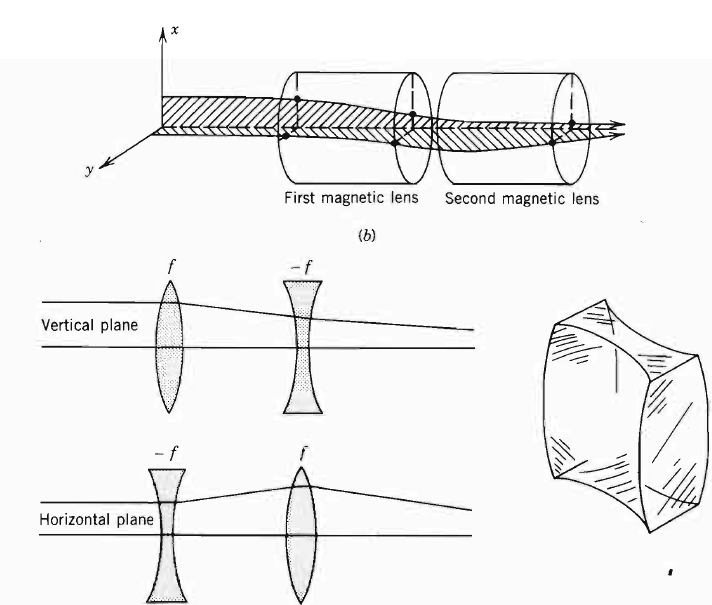
\includegraphics[scale=0.6]{analogy}
        \caption{Analogía entre los lentes magnéticos y los lentes ópticos}
        \label{fig:analogy}
    \end{figure}

    En la \cref{fig:analogy} se muestra esta analogía puesta en acción. En lugar de lentes ópticas, se usan campos magnéticos, y nos podemos referir a estos como lentes magnéticas (para continuar con la analogía) las cuales cambian la dirección de la trayectoria de la partícula, y con diferentes configuraciones de imanes se puede lograr deflectar el haz de partículas. Esto en particular se logra usando cuadrupolos magnéticos, donde en un eje se puede enfocar y en el otro desenfocar.

    En el cuadrupolo magnético, el haz de partículas cargadas se guía por la ley de Lorentz generalizada

    \begin{equation*}
      \vect{F} = q(\vect{E} + \vect{v} \mul \vect{B})
    \end{equation*}

    Y esta desviación es perpendicular a la trayectoria de la partícula, tal que en las direcciones $x$ y $y$ las componentes del campo magnético son de la forma \(B_{x} = by\) y \(B_{y} = bx\), mientras que las componentes de la fuerza de Lorentz son

    \begin{align*}
      F_{x} &= -qv_{z}B_{y} = -qv_{z}bx = -kx,\\
      F_{y} &= qv_{z}B_{x} = qv_{z}by = ky.
    \end{align*}

    \section{Tipos de aceleradores}

    \subsection{Aceleradores lineales o linac}

    Los aceleradores lineales como su nombre lo indica aceleran las partículas en trayectorias rectas. El funcionamiento de estos aceleradores está basado en el principio de resonancia.

    En 1924, G. Ising propuso acelerar partículas con una serie de campos eléctricos oscilantes y en 1929 esta idea fue llevada a la práctica por Wider\o e, propuso una estructura compuesta de una serie de tubos cilíndricos (ver~ \cref{fig:linac}), llamados tubos de deriva (\emph{drift tubes} por su nombre en inglés) que reciben la señal de una guía de ondas y las cavidades alternan su campo. A bajas energía las cavidades son de distinto tamaño, de forma que en la cavidad el paquete de partículas se acelera hacia adelante. Durante el tiempo que están en la cavidad su sentido se mantiene, pero una vez dentro de los tubos de deriva la dirección del campo se invierte, de tal manera que en las cavidades vecinas inmediatas sientan nuevamente una aceleración hacia adelante.\cite{conte2008introduction,moreno2020aceleradores} Una limitante de este tipo de aceleradores es que para distancias mayores la curvatura de la Tierra interfiere, además de que se requieren voltajes cada vez mayores.

    \begin{figure}[!htb]
        \centering
        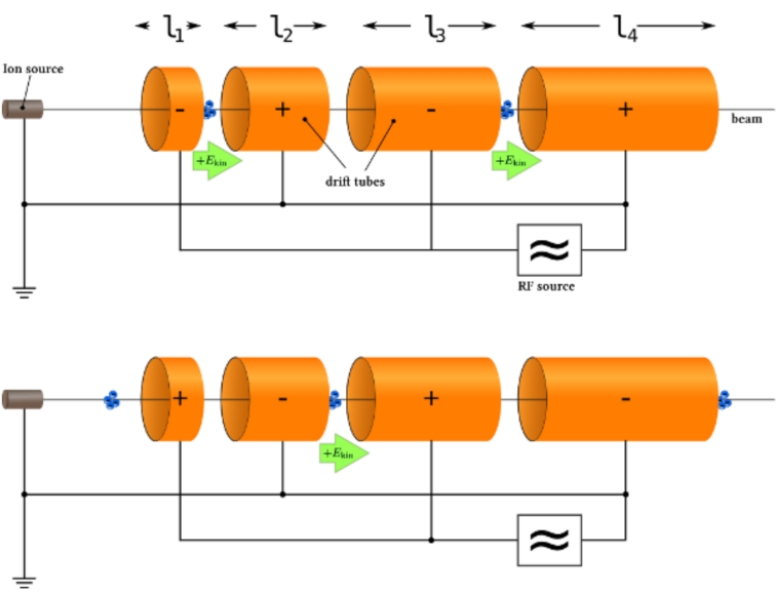
\includegraphics[scale=0.6]{linac}
        \caption{Esquema del principio del funcionamiento de un acelerador lineal.\cite{moreno2020aceleradores}}
        \label{fig:linac}
    \end{figure}

    Entre los aceleradores lineales tenemos a los aceleradores de tipo Van de Graaff.

    \subsubsection{Acelerador Van de Graaff}

    Sabemos que la energía de un partícula acelerada por una diferencia de potencial es directamente proporcional al voltaje aplicado, por lo que la construcción inteligente de una fuente de voltaje es de crucial importancia. Este es el principio en el que se basan los aceleradores Van de Graaff (VDG), denominados así en honor de su inventor Robert Van de Graaff en la Universidad de Princeton, quien en el año 1929 desarrolló un método para generar alto voltaje.\cite{das2003introduction}
    
    El principio por el cual se acelera una partícula cargada es haciéndola ``caer'' a través de una diferencial de potencial \(V\), lo cual provoca que adquiera una energía cinética de \(qV\). En el VDG se aceleran las carga por un método mecánico y electrostático. Se generan iones y se mueven mediante una banda transportadora hasta la terminal, usando voltajes del orden de \qtyrange{20}{30}{\kV}, la banda se mueve por medio de un motor hasta una terminal donde es recolectada por agujas metálicas que lo distribuyen por una amplia área metálica. Así se tiene una región cargada negativamente, dentro de la cual se producen iones y por la repulsión coulombiana salen disparados fuera de esta región.\cite{krane1991introductory} (ver \cref{fig:VDG})
    
    \begin{figure}[htb]
        \centering
        \includegraphics[scale=0.5]{VDG}
        \caption{Esquema de un acelerador Van de Graaff.\cite{Hinterberger:1005042}}
        \label{fig:VDG}
    \end{figure}

    \subsubsection{Pelletron}

    El acelerador Pelletron (ver \cref{fig:pelletron}) es similar al VDG, sin embargo las bandas transportadoras fueron sustituidas por cadenas de anillos transportadores de carga, que solucionan los múltiples dificultadas que presentaban, de entre las cuales destacan la inestabilidad del voltaje terminal y la susceptibilidad por daño debido a chispas.\cite{herb1971pelletron}

    Las cadenas del Pelletron están formadas pellets (perdigones y, de ahí su nombre) de metal conectados por algo un material aislante, en particular el nylon. Los perdigones se cargan debido a la influencia de un campo eléctrico. Para iones positivos, el campo eléctrico entre el electrodo inductor polarizado negativamente y la polea que le quita electrones a los perdigones mientras se encuentran en contacto con la polea conectada a tierra. Y puesto que los perdigones aún se encuentran dentro del campo eléctrico conforme se apartan de la polea, mantiene una carga total positiva. Después la cadena transporta la carga a la terminal de alto voltaje, donde el proceso opuesto toma lugar. La transferencia de la carga es controlada por inductores en forma de U, que se encuentran colocadas de tal manera que se evite la generación de chispas.\cite{Hinterberger:1005042}

    Una vez que la carga alcanza la terminal, la cadena pasa por un electrodo supresor polarizado negativamente lo cual previene la generación de chispas.
    
    \begin{figure}[htb]
        \centering
        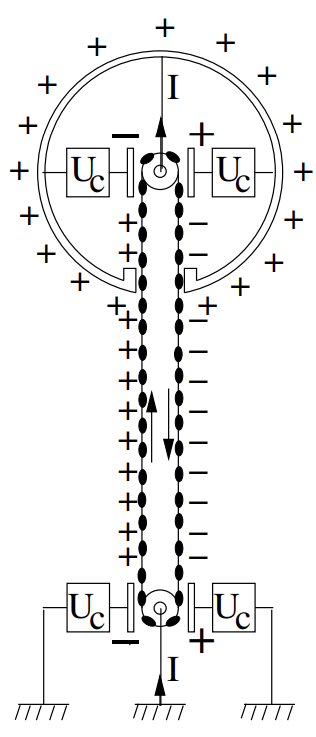
\includegraphics[scale=0.5]{pelletron}
        \caption{Esquema del Pelletron.\cite{Hinterberger:1005042}}
        \label{fig:pelletron}
    \end{figure}

    \subsubsection{Tandem}

    La concepción del acelerador Tandem (ver \cref{fig:tandem}) fue debida al objetivo de lograr haces con energías aún mayores que las logradas por un VDG. El Tandem utiliza la termina de voltaje dos veces para lograr energías mayores dos veces o más a las que se obtendrían con una sola aceleración. Iones negativos producidos por una fuente de iones apropiada \(I\) son aceleradores de una terminal conectada a tierra a una positivamente cargada. Dentro de la terminal se encuentra un \emph{stripper} que remueve electrones de los iones negativos. Ahí mismo los iones experimentan una segunda aceleración al dejar la terminal y viajan a otra terminal conectada a tierra. Las energías cinéticas \(T\) del haz depende de la carga de los iones positivos,

    \begin{equation*}
      T = (\e + q)U,
    \end{equation*}

    donde \(\e\) es la carga de un ion negativamente cargado y la carga \(q\) de los iones puede ser múltiplos de \(\e\).

    Los aceleradores Tandem más poderosos son capaces de alcanzar voltajes de hasta \qty{20}{\mega\V} y \qty{30}{\mega\V}.

    \begin{figure}[htb]
        \centering
        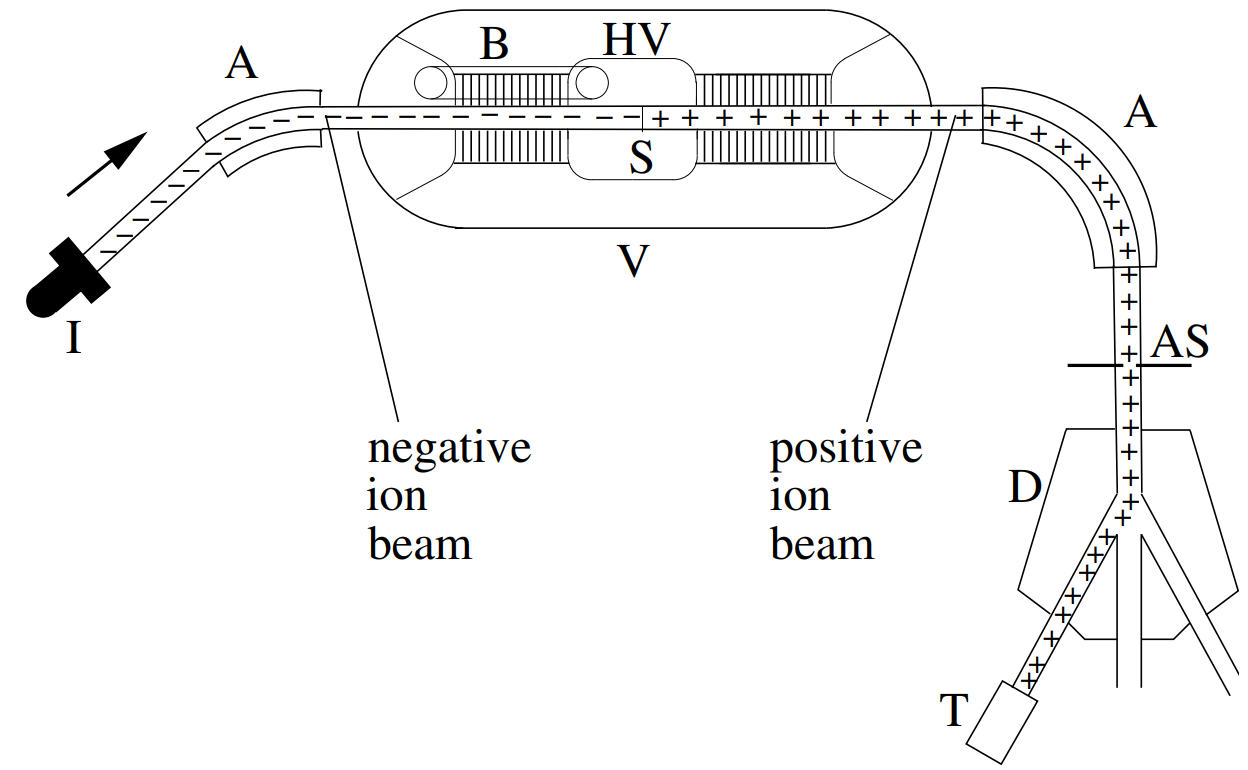
\includegraphics[scale=0.5]{tandem}
        \caption{Esquema de un acelerador Tandem.\cite{Hinterberger:1005042}}
        \label{fig:tandem}
    \end{figure}

    \subsection{Aceleradores circulares}

    \subsubsection{Ciclotrón}

    Una alternativa a los linac son los dispositivos circulares en los cuales un haz de partículas recorre el dispositivo varias veces, recibiendo un pequeño incremento de voltaje con cada ciclo completado de tal forma que la partícula alcance una energía que se encuentre en el rango de \unit{\MeV}.

    Uno de los aceleradores circulares más simples es el conocido como \textbf{ciclotrón}, la idea fue concebida por Ernest Lawrence en la Universidad de California en Berkley. Usando del principio de resonancia se construye un acelerador cíclico, cuya zona de aceleración está en el diámetro del círculo formado a partir de dos secciones metálicas en forma de \(D\) huecas a las que se les aplica un alto voltaje oscilante de alta frecuencia. Dentro de las Des huecas, las partículas hacen una trayectoria semicircular a velocidad (casi) constante producida por un campo magnético uniforme perpendicular a estas secciones. Cuando las partículas llegan al límite de separación entre las Des, la polaridad del potencial entre ellas se cambia y las partículas son aceleradas en el espacio entre ellas.

    Para verificar lo anterior lo hacemos mediante una aproximación clásica, la fuerza de Lorentz de una órbita circular, \(qvB\),  provee la suficiente aceleración centrípeta. para mantener el movimiento circular, tal que

    \begin{equation*}
      F = qvB = \dfrac{mv^{2}}{r}
    \end{equation*}

    Y sabemos que la frecuencia angular para un movimiento circular a velocidad constante es

    \begin{equation*}
      \omega = \dfrac{v}{r}.
    \end{equation*}

    Expresamos la frecuencia como

    \begin{equation*}
      \nu = \dfrac{\omega}{2\pi} = \dfrac{1}{2\pi}\left(\dfrac{q}{m}\right)B.
    \end{equation*}

    Que es la frecuencias del ciclotrón o la frecuencia de resonancia del ciclotrón.

    La energía máxima que puede alcanzar una partícula extraída del ciclotrón a un radio R es:

    \begin{equation*}
      T = \dfrac{1}{2}mv^{2}_{\text{máx}} = \dfrac{1}{2m}q^{2}B^{2}R^{2}.
    \end{equation*}

    Sin embargo, este acelerador ya no funciona para poder acelerar a velocidades relativista, debido a que la frecuencia necesaria sería altísima.

    \subsubsection{Sincrotón}

    Para este tipo de aceleradores se sigue el mismo principio del funcionamiento de los aceleradores lineares, pero acomodado en un círculo, y en lugar de un solo campo magnético ahora se ponen campos magnéticos pequeños en distintos puntos de la aceleración.
    
    \section{Aplicaciones}
    
    Las aplicaciones de los aceleradores tienen sus raíces en la física nuclear, pero con el paso del tiempo se han ido diversificando. Sus aplicaciones son multidisciplinarias y van desde el arte hasta la zoología.\cite{amaldi2000importance}
    
    Por ejemplo, en las artes uno puede considerar el trabajo realizado en el ``Accélérateur Grand Louvre d'analyse élémentaire'' (AGLE), un acelerador Pelletron que se encuentra en el museo del Louvre en París, Francia. Este acelerador se usó para analizar un cuadro realizado alrededor del año 1450 que se le atribuía al pintor Pisanello a través de la técnica PIXE.

    Sin embargo, a continuación hablaremos con un poco más de detalle de las aplicaciones de los aceleradores en la industria, la agricultura y la medicina.
    
    \subsection{Usos en la industria}

    En la industria\cite{chernyaev2014particle}, los aceleradores de iones son de bajas energías y están restringidos a un rango de unos cientos de electronvolts hasta \qty{500}{\keV}; mientras que las energías para los aceleradores de protones se encuentra entre los \qty{0.5}{\MeV} hasta los \qty{70}{\MeV}. 

    Por un lado, las instalaciones que proveen energías en el rango \qtyrange{70}{300}{\keV} son usadas para coser polímeros, la purificación de líquidos y gases, la esterilización de superficies y el calentamiento de plasma en fusión termonuclear.

    Por el otro, los acelerados que proveen haces con energías en el rango \qty{300}{\keV} y \qty{5}{\MeV} son usados para fabricar cables y alambres, producción de espuma de polietileno, vulcanizar componentes de neumáticos y en la purificación de drenaje. Mientras que los aceleradores de mayor energía, que se encuentra en el rango de \qtyrange{5}{10}{\MeV} son usados en la esterilización de equipo médico, entre muchas otras más.

    \subsection{Agricultura e industria alimentaria}

    Las fuentes de radiación ionizante han sido utilizados en la industria alimentaria y en la agricultura por más de 70 años. Se ha usado para esterilizar y desinfectar productos, así como para la prevención de la germinación de semillas para almacenamiento y para crear variaciones de cultivos con características mejoradas.

    \subsection{Uso de los aceleradores en la medicina}

    El uso de los aceleradores en la medicina comenzó casi desde su invención, ya que desde 1937 se usaban para el tratamiento de enfermedades oncológicas, así como en la radioterapia.

    Conforme la tecnología fue avanzando, se logró tener aceleradores en hospitales. Los ciclotrones son usados para producir isótopos que se utilizan para la tomografía por emisión de positrones (PET) y para la tomografía computarizada de emisión monofotónica (SPECT).

    \pagebreak
    \printbibliography
\end{document}